\documentclass[a4paper]{article}

\usepackage[utf8]{inputenc}
\usepackage[T1]{fontenc}
\usepackage{textcomp}
\usepackage{listings}
\usepackage{lmodern}
\usepackage{amsfonts}
\usepackage{titling}
\usepackage{lipsum}
\usepackage[left=1in, right=1in, bottom=1in, top=1in]{geometry}
\usepackage{amsthm}
\usepackage{tcolorbox}
\usepackage{hyperref}
\usepackage{xcolor}
\usepackage{graphicx}
\usepackage{makeidx}
\usepackage{tikz}
\usepackage{cases}
\usepackage{apacite}
\usepackage{tkz-berge}
\usepackage{url}
\usepackage{tgtermes}
\usepackage{sectsty}
\usepackage{subcaption}
\usepackage{setspace}
\usepackage{float}
\usepackage{amsmath, amssymb}


% figure support
\usepackage{import}
\usepackage{xifthen}
\pdfminorversion=7
\usepackage{pdfpages}
\usepackage{transparent}
\usepackage{color}
\newcommand{\incfig}[2][1]{%
    \def\svgwidth{#1\columnwidth}
    \import{./figures/}{#2.pdf_tex}
}

%mathstyling
\theoremstyle{plain}
\newtheorem{thm}{Theorem}[section]
\newtheorem{lem}[thm]{Lemma}
\newtheorem{prop}[thm]{Proposition}
\newtheorem*{cor}{Corollary}

\theoremstyle{definition}
\newtheorem{defn}{Definition}[section]
\newtheorem{conj}{Conjecture}[section]
\newtheorem{exmp}{Example}[section]
\newtheorem{axiom}{Axiom}
\theoremstyle{remark}
\newtheorem*{rem}{Remark}
\newtheorem*{note}{Note}

\definecolor{darkgreen}{rgb}{0.0, 0.5, 0.0}

\pdfsuppresswarningpagegroup=1
\lstset{
tabsize = 4, %% set tab space width
showstringspaces = false, %% prevent space marking in strings, string is defined as the text that is generally printed directly to the console
numbers = left, %% display line numbers on the left
commentstyle = \color{darkgreen}, %% set comment color
keywordstyle = \color{blue}, %% set keyword color
stringstyle = \color{red}, %% set string color
rulecolor = \color{black}, %% set frame color to avoid being affected by text color
basicstyle = \small \ttfamily , %% set listing font and size
breaklines = true, %% enable line breaking
numberstyle = \tiny,
  frame=none,
  xleftmargin=2pt,
  stepnumber=1,
  belowcaptionskip=\bigskipamount,
  captionpos=b,
  escapeinside={*'}{'*},
  language=haskell,
  tabsize=2,
  emphstyle={\bf},
  showspaces=false,
  columns=flexible,
  showstringspaces=false,
  morecomment=[l]\%,
}
\begin{document}
	\begin{titlepage}
	\begin{center}
	\large
	University of Warwick \\
	Department of Computer Science \\
	\huge
	\vspace{50mm}
	\rule{\linewidth}{0.5pt} \\
	CS241 \\
	\vspace{5mm}
	\Large
	Operating Systems and Computer Networks
	\rule{\linewidth}{0.5pt}
	\vspace{5mm}
	\begin{figure}[H]
	\centering
	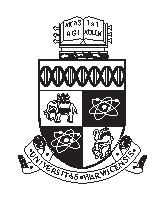
\includegraphics[width=0.4\textwidth]{crest_black.eps}
	\end{figure}
	\vspace{37mm}
	Cem Yilmaz \\
	\today
	\end{center}
	\end{titlepage}
	\tableofcontents
	\newpage
	\section{Introduction}
	\subsection{What is an operating system?}
	There is no universally accepted definition, however, a broad definition would be as follows
	\begin{tcolorbox}[colback=black!3!white,colframe=black!60!white,title=\begin{defn}Operating system \label{Operating system}\end{defn}]
	A software acting as an intermediary between the user of a device and the hardware of a device. Examples include, but are not limited to, PCs, laptops, phones, cars, airplanes, etc.
	\end{tcolorbox}
	A computer system hardware resources include CPU, Memory, I/O devices and storage. The OS is responsible for allocating these resources to user processes and control their execution. Th e goal is to avoid failures and errors e.g., two programs writing in the same memory.
	\subsubsection{Program Execution}
	The system must be able to load a program into memory, execute that program and stop that program either normally or abnormally.
	\subsubsection{I/O Operations}
	While running, a program may require to perform I/O. For example, display something to the terminal, take input from keyboard. \\
	For efficiency and protection, users cannot control devices directly. Instead, the OS controls I/O devices through device drivers and interrupts. More efficient because users do not need to write codes to perform I/O and more secure because multiple programs cannot access the same I/O simultaneously. 
	\subsubsection{File System Management}
	A program needs to read and write files and directories, perform additional operations such as copy and move, and finally, these functions may be subject to permission management. The OS system provides system calls to achieve these.
	\subsubsection{Error handling}
	The operating system needs to be detecting and correcting errors constantly. Errors may occur in hardware e.g., failure of cpu, memory and I/O devices or user programs e.g., arithmetic overflow, illegal memory access. 
	\subsubsection{Resource Allocation}
	When there are multiple users or multiple jobs running at the same time, resources must be allocated to each of them. In scheduling CPU jobs, the OS must consider the speed of the processor, number of processors available, jobs to be executed etc.
	\subsubsection{Accounting}
	It is necessary to keep track of which processes are running and how much resources they consume. Such information may be used for system administration or billing purposes e.g., clouds. The operating system gathers this information through control blocks.
	\subsubsection{Protection and Security}
	When separate processes execute concurrently they should not be able to interfere with other processes or with the operating system itself. Security of the system from outside attacks is just as important.
	\subsection{What is the Kernel?}
	\begin{tcolorbox}[colback=black!3!white,colframe=black!60!white,title=\begin{defn}Kernel \label{Kernel}\end{defn}]
	Kernel is the core of an operating system. It is loaded into the main memory at system startup and is a process that runs at all times in the computer. There are certain functions which only a kernel can perform, e.g., memory management, process scheduling and file handling.
	\end{tcolorbox}
	\subsubsection{Kernel Space vs User Space}
	Kernel space is part of the memory where kernel executes. User space is the section of memory where user processes run. Kernel space is kept protected from user space. Kernel space can be accessed via user processes through system calls. These calls perform services like I/O operations or process creation.
	\subsubsection{System Calls}
	When a user process requires a service from the kernel e.g., reading from a file or reading to a file, it invokes a system call. System calls are required since user processes cannot perform certain privileged operations. System calls are low-level functions provided by the operating system. They provide a consistent interface for common operations. E.g., read(), write()
	\subsubsection{Dual mode operation}
	A mechanism to distinguish between OS operations and user operations. Hardware operates in two modes: user mode and kernel mode. Mode bit (0 or 1) indicates a kernel or a user mode. Some instructions are designated as privileged, only executable in kernel mode. System calls by a user asking the OS to perform some function changes from user mode to kernel mode. Return from a system call recalls.
\end{document}
